% ****** Start of file apssamp.tex ******
%
%   This file is part of the APS files in the REVTeX 4.1 distribution.
%   Version 4.1r of REVTeX, August 2010
%
%   Copyright (c) 2009, 2010 The American Physical Society.
%
%   See the REVTeX 4 README file for restrictions and more information.
%
% TeX'ing this file requires that you have AMS-LaTeX 2.0 installed
% as well as the rest of the prerequisites for REVTeX 4.1
%
% See the REVTeX 4 README file
% It also requires running BibTeX. The commands are as follows:
%
%  1)  latex apssamp.tex
%  2)  bibtex apssamp
%  3)  latex apssamp.tex
%  4)  latex apssamp.tex
%
\documentclass[%
 reprint,
%superscriptaddress,
%groupedaddress,
%unsortedaddress,
%runinaddress,
%frontmatterverbose, 
%preprint,
%showpacs,preprintnumbers,
%nofootinbib,
%nobibnotes,
%bibnotes,
 amsmath,amssymb,
 aps,
%pra,
%prb,
%rmp,
%prstab,
%prstper,
%floatfix,
]{revtex4-1}

\usepackage{graphicx}% Include figure files
\usepackage{subfigure}
\usepackage{multirow}
\usepackage{array}
\usepackage{dcolumn}% Align table columns on decimal point
\usepackage{bm}% bold math
%\usepackage{hyperref}% add hypertext capabilities
%\usepackage[mathlines]{lineno}% Enable numbering of text and display math
%\linenumbers\relax % Commence numbering lines

%\usepackage[showframe,%Uncomment any one of the following lines to test 
%%scale=0.7, marginratio={1:1, 2:3}, ignoreall,% default settings
%%text={7in,10in},centering,
%%margin=1.5in,
%%total={6.5in,8.75in}, top=1.2in, left=0.9in, includefoot,
%%height=10in,a5paper,hmargin={3cm,0.8in},
%]{geometry}

\usepackage{xeCJK}
\setCJKmainfont[ItalicFont={KaiTi}, BoldFont={KaiTi}]{KaiTi}
\usepackage{textcomp}
\usepackage{chemfig}
\usepackage[version=4]{mhchem}
\usepackage{fontspec}
\usepackage{listings}
\usepackage{xcolor}
\usepackage{xcolor} % 定制颜色
\definecolor{mygreen}{rgb}{0,0.6,0}
\definecolor{mygray}{rgb}{0.5,0.5,0.5}
\definecolor{mymauve}{rgb}{0.58,0,0.82}
\lstset{
backgroundcolor=\color{white},      % choose the background color
basicstyle=\footnotesize\ttfamily,  % size of fonts used for the code
columns=fullflexible,
tabsize=4,
breaklines=true,               % automatic line breaking only at whitespace
captionpos=b,                  % sets the caption-position to bottom
commentstyle=\color{mygreen},  % comment style
escapeinside={\%*}{*)},        % if you want to add LaTeX within your code
keywordstyle=\color{blue},     % keyword style
stringstyle=\color{mymauve}\ttfamily,  % string literal style
frame=single,
rulesepcolor=\color{red!20!green!20!blue!20},
% identifierstyle=\color{red},
language=Mathematica,
}

\usepackage[normalem]{ulem}

\newcommand{\chuhao}{\fontsize{42pt}{44.9pt}\selectfont}    % 初号, 1.5倍行距
\newcommand{\xiaochu}{\fontsize{30pt}{40pt}\selectfont}    % 小初, 1.5倍行距
\newcommand{\yihao}{\fontsize{26pt}{36pt}\selectfont}    % 一号, 1.4倍行距
\newcommand{\erhao}{\fontsize{22pt}{28pt}\selectfont}    % 二号, 1.25倍行距
\newcommand{\xiaoer}{\fontsize{18pt}{18pt}\selectfont}    % 小二, 单倍行距
\newcommand{\sanhao}{\fontsize{16pt}{24pt}\selectfont}    % 三号, 1.5倍行距
\newcommand{\xiaosan}{\fontsize{15pt}{22pt}\selectfont}    % 小三, 1.5倍行距
\newcommand{\sihao}{\fontsize{14pt}{21pt}\selectfont}    % 四号, 1.5倍行距
\newcommand{\sihaox}{\fontsize{14pt}{28pt}\selectfont}    % 四号, 1.5倍行距
\newcommand{\banxiaosi}{\fontsize{13pt}{19.5pt}\selectfont}    % 半小四, 1.5倍行距
\newcommand{\xiaosix}{\fontsize{12pt}{24pt}\selectfont} 	% 小四, 1.5倍行距
\newcommand{\xiaosi}{\fontsize{12pt}{18pt}\selectfont}     
\newcommand{\dawuhao}{\fontsize{11pt}{11pt}\selectfont}    % 大五号, 单倍行距
\newcommand{\wuhao}{\fontsize{10.5pt}{10.5pt}\selectfont}    % 五号, 单倍行距
\newcommand{\xiaowu}{\fontsize{9pt}{9pt}\selectfont}    % 五号, 单倍行距

%\usepackage[fntef]{ctexcap}
%\CTEXsetup[number={\chinese{section}、},format={\Large\bfseries}]{section}
\setCJKfamilyfont{fangsong}{FangSong}                      %仿宋2312 fs  
\newcommand{\fangsong}{\CJKfamily{fangsong}}  

\usepackage{wrapfig}
\usepackage{fancyhdr}
\usepackage{fancybox}   






\newcommand{\bra}[1]{\langle #1 |}
\newcommand{\ket}[1]{| #1 \rangle}
\newcommand{\bracket}[2]{\langle #1 | #2 \rangle}
\newcommand{\bracketl}[3]{\langle #1 | #2 | #3 \rangle}
\newcommand{\func}{\mathrm \,}
\newcommand{\define}[2]{
	\begin{definition}
	\begin{description}
	\item[#1]
	#2
	\end{description}
	\end{definition}
}

\newcommand{\sch}{Schr\"odinger}
\newcommand{\grad}{\nabla}
\newcommand{\ueq}{\neq}
\newcommand{\celsius}{\ensuremath{^\circ\hspace{-0.09em}\mathrm{C}}}
\newcommand{\unit}[2]{$#1 \, \mathrm{#2}$}

\begin{document}

%\preprint{APS/123-QED}

\title{Approximation of viscosity average molecular weight of polyethlene glycol}% Force line breaks with \\
%\thanks{A footnote to the article title}% give thanks

\author{Rui Li}
 %\altaffiliation[Also at ]{Physics Department, XYZ University.}%Lines break automatically or can be forced with \\
%\author{Second Author}%
%\email{3160102098@zju.edu.cn}
\affiliation{%
 Qiushi science class (chemistry)\\
 Chu Kochen Honor College
}%

%\collaboration{MUSO Collaboration}%\noaffiliation

\author{Zong Wei Huang}
% \homepage{http://www.Second.institution.edu/~Charlie.Author}
%\affiliation{
% Second institution and/or address\\
% This line break forced% with \\
%}%
\affiliation{
Qiushi science class (chemistry)\\
 Chu Kochen Honor College
}%
%\author{Delta Author}
%\affiliation{%
% Authors' institution and/or address\\
% This line break forced with \textbackslash\textbackslash
%}%

%\collaboration{CLEO Collaboration}%\noaffiliation

%\date{\today}% It is always \today, today,
             %  but any date may be explicitly specified

\begin{abstract}
The viscosity average molecular weight of polyethelene glycol is approximated using Mark-Houwink's empirical equation, and intrinsic viscosity is obtained using Huggins' equation and Kramer's equation respectively. The reliablity of thermostat is investigated in detail, exploring several factors that affect the fluctuation of the temperature. Programs are also utilized to reveal some basic relation between these factors, as well as indicating some plausible improvements for further stabilization of the temperature.
\begin{description}
\item[Keywords]
viscosity average molecular weight, polyethelene glycol, thermostat
\end{description}
\end{abstract}

%\pacs{Valid PACS appear here}% PACS, the Physics and Astronomy
                             % Classification Scheme.
%\keywords{Suggested keywords}%Use showkeys class option if keyword
                              %display desired
\maketitle

\tableofcontents

\section{The fluctuation of temperature in thermostat}
The fluctuation of temperature is a key factor in measuring viscosity of liquids, whose huge dependence on temperature greatly affects whether a strong linear relation between viscosity and density can be obtained. The characteristics of the fluctuation curves are investigated in detail using computational methods.

\subsection{Simulations}
Heat flow satisfies
\begin{equation}
\frac{d \mathbf{q}}{dt} = - D_f \nabla T,
\end{equation}
while the temperature at a point also satisfies
\begin{equation}
\frac{d T}{dt} = C_V \iint \mathbf{q}\cdot d\mathbf{\sigma}.
\end{equation}
In one-dimension discrete model, the equations reduce to
\begin{equation}
\begin{cases}
\frac{\Delta q}{\Delta t} \sim D_f \frac{T(x+\Delta x)+T(x-\Delta x)-2T(x)}{2\Delta x}\\
\Delta  T(x) \sim \frac{\Delta q /\Delta t}{C_V}\Delta t
\end{cases}
\end{equation}

The exact model set up using \emph{Julia} includes a linearly heated cell, a cell whose temperature is fixed to the room temperature, and a temperature measuring cell which controls heating through comparing its temperature measured to the target temperature set initially.
\begin{equation}
\begin{cases}
\Delta T/\Delta t |_{\text{heat cell}} = k \\
T(\text{wall}) = T_{\text{room}}
\end{cases}
\end{equation}
Specifically, the model adopts 30 cells and $\Delta t$ is set to 0.01 s\footnote{The model is relatively sensitive to the value of $\Delta t$, which mainly determines the numerical unstability of the whole simulation, namely the fluctuation of the data itself.}, and all the simulations go through 100,000 iterations.

The relation between fluctuation and heating speed is investigated, whose result is shown in Fig.\ref{heatspeed}, where a sharp increase can be observed at initial stage. This can easily be attributed to the `delay' of measurement of temperature, derived from the time inquired for the heat flow to `pass over' the measuring cell. A non-sinusoidal behavior is also revealed, which results from the unequality between heating speed and cooling speed. At temperature relatively close to the room temperature results in lower speed of cooling, which leads to more time spent in reducing the exceeded temperature. Fig.\ref{targettemp} further explains this result, introducing the fact that the fluctuation become sinusoidal as the target temperature increases. Fig.\ref{heatspeed} also indicates higher frequency,smaller amplitude of the fluctuation and less to time spent to achieve such a state, when lower speed of heating is set.

\begin{figure}
\centering
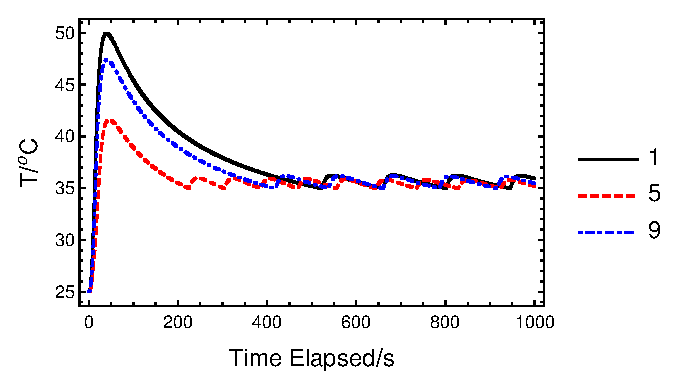
\includegraphics[width=0.4\textwidth]{figures/heatspeed.eps}
\caption{The flctuation curves having heating speed as the main variant. The numbers in legends shown represent the heating speed in the simulations.}
\label{heatspeed}
\end{figure}

Fig.\ref{targettemp} further shows a slight difference of frequency and amplitude among different target temperature, which is also derived from the different speed of cooling. The same reason can be applied to the facts that the mean of the temperature is universally higher than the target temerature, and that the mean temperature gradually approaches the target temperature when it increases.

\begin{figure}
\centering
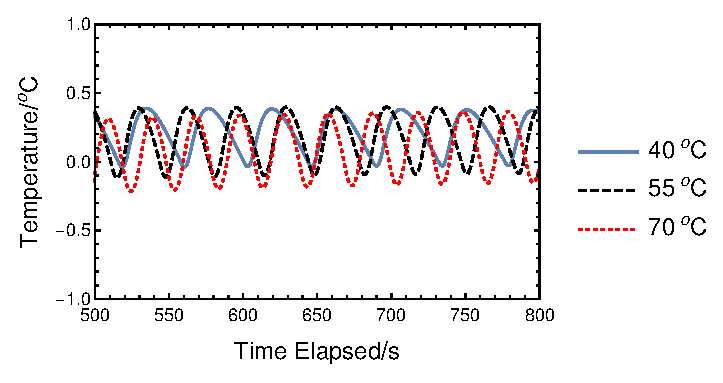
\includegraphics[width=0.4\textwidth]{figures/targettemp.eps}
\caption{The flctuation curves having target temperature as the main variant. The y-axis represents the deviation from the target temperature.}
\label{targettemp}
\end{figure}

Fig.\ref{tempdetect} helps draw the conclusion that smaller distance between heat source and temperature measuring device leads to better stability of temperature around the measuring device. From another perspective, the trend of the curve in the cell away from both the heat source and the measuring cell differs from cells between them, namely that rather than fluctuating it shows a converging behavior towards target temperature. This might indicate a better position in thermostats for thermo-sensitive experiments.

\begin{figure}
\centering
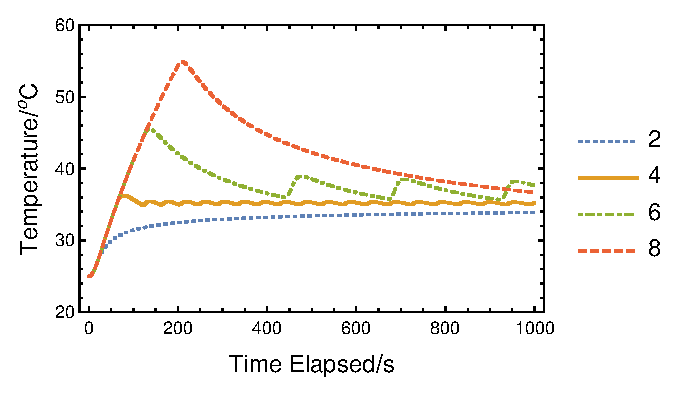
\includegraphics[width=0.4\textwidth]{figures/tempdetect.eps}
\caption{The flctuation curves having the position of the measuring cell as the main variant, concerning temperature of the third cell. The numbers in legends represent the index of the measuring cell in the array.}
\label{tempdetect}
\end{figure}

Dual heat sources might not be appropriate for stabilizing the temperature in thermostats, as shown in Fig.\ref{singledual}. Even equating the power of the heat source does not restrict the amplitude of fluctuation. Lower frequency might also results in worse experimental conditions. A snapshot from the dual-heat-source model shown in Fig.\ref{dualsnapshot} denies the mind-set that a relatively mild decrease can be obtained between the two heat sources, which might results from quicker heat flow and then easier excess of heat supply.

\begin{figure}
\centering
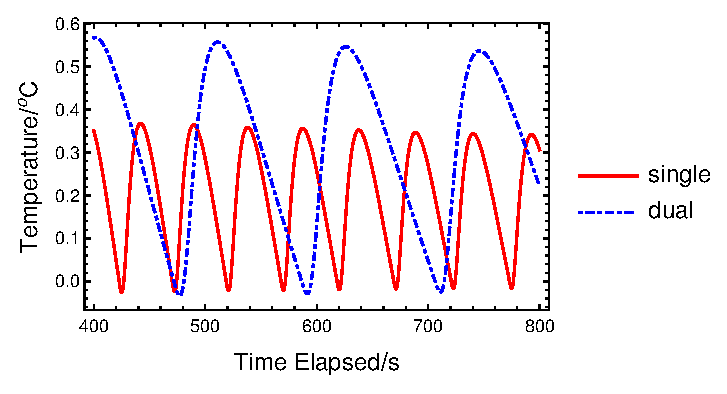
\includegraphics[width=0.4\textwidth]{figures/singledualcomp.eps}
\caption{The flctuation curves concerning whether there is single heat source or dual. The other heat source is set at $7^\text{th}$ cell and the heating speed of both heat sources is set half of it in single-heat-source model.}
\label{singledual}
\end{figure}

\begin{figure}
\centering
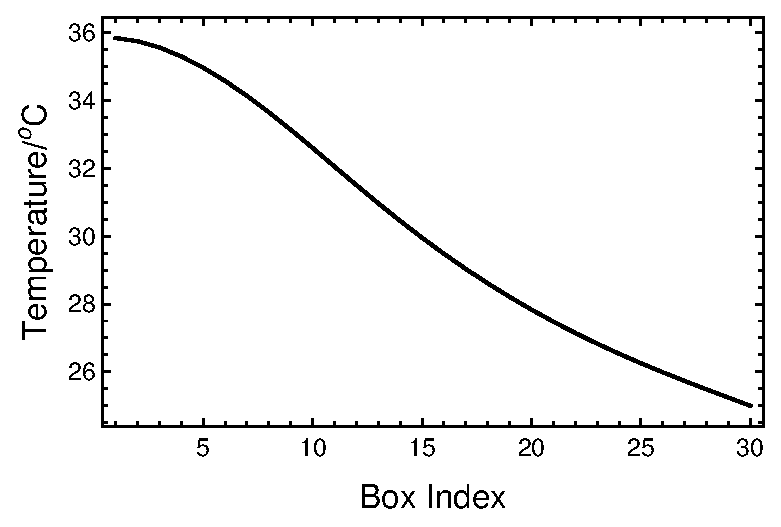
\includegraphics[width=0.35\textwidth]{figures/dualheatsnapshot.eps}
\caption{A snapshot from the dual-heat-source model}
\label{dualsnapshot}
\end{figure}

\subsection{Experimental Results}
Fig.\ref{heating} presents the heating process, most characteristics of which have been indicated by numerical simulations, including an excess of temperature before fluctuation, as well as non-sinusoidal behavior. The asymmetry of the fluctuation curve remsembles the one provided in simulations, which further validates the computational model. Fig.\ref{volt} also reveals the relation between heating speed and the fluctuation's amplitude and frequency, which is the same as deduced in simulations. Smaller amplitude and higher frequency in experiments are attributed to better thermal conduct than in simulations. 

0.04 \celsius~of deviation in thermostat under 110 V indicates that the following experiment, namely the measurement of viscosity of polymer's solution and approxmation of polymer's molecular weight, is executed under relatively stable thermal conditions.
\begin{figure}
\centering
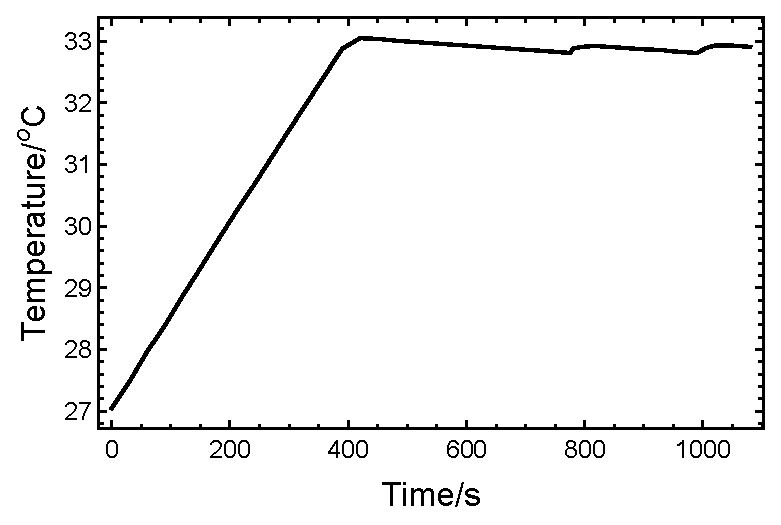
\includegraphics[width=0.35\textwidth]{figures/Heating.eps}
\caption{Heating of water with heater under voltage of 220 V and target temperature set at 32 \celsius}
\label{heating}
\end{figure}

\begin{figure}
\centering
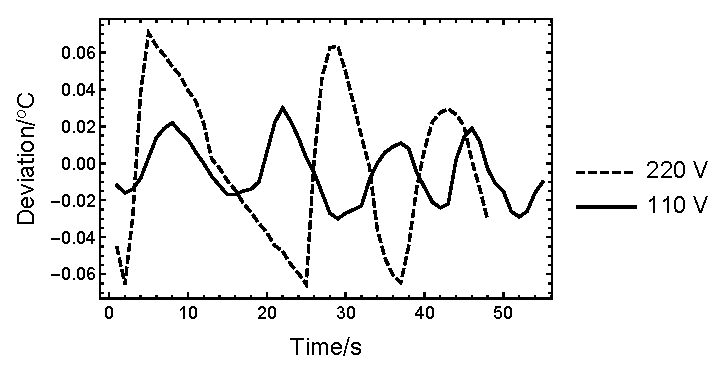
\includegraphics[width=0.4\textwidth]{figures/DifVoltDeviation.eps}
\caption{Fluctuation of temperature under heating voltage of 220 V and 110 V}
\label{volt}
\end{figure}

\section{The measurement of viscosity of polymer's solution, and approxmation of polymer's molecular weight}

The temperature of the thermostat is set to 35 \celsius in the experiment, and the fluctuation has been proved to be trivial. Table.\ref{groupA} and Table.\ref{groupB} contain the experimental results, and Table.\ref{eta} concludes the $[\eta]$ calculated from two groups and two methods. The density of polyethylene glycol solution adopts 'unit' as its unit proportional to standard unit, causing no confusion nor error in the approximation of $[\eta]$. Fig.\ref{etafig} shows the linear fitting of the data. It is defined that
\begin{equation*}
\begin{cases}
[\eta]' = \frac{\eta_\text{sp}}{c}\\
[\eta]' = \frac{\eta_\text{r}}{c}
\end{cases}
\end{equation*}


\begin{table}
\centering
\caption{Group A}
\begin{tabular}{cccc}\hline
density/unit & $t$/s & $\eta_\text{r}$ & $\eta_\text{sp}$ \\\hline
0. & 80.48 & 1.000 & 0.000 \\
1. & 89.94 & 1.118 & 0.118 \\
2. & 100.7 & 1.252 & 0.252 \\\hline
\end{tabular}
\label{groupA}
\end{table}

\begin{table}
\centering
\caption{Group B}
\begin{tabular}{cccc}\hline
density/unit & $t$/s & $\eta_\text{r}$ & $\eta_\text{sp}$ \\\hline
0. & 71.12 & 1.000 & 0.000 \\
3. & 99.43 & 1.398 & 0.398 \\
4. & 110.7 & 1.557 & 0.557 \\
5. & 121.5 & 1.709 & 0.709 \\\hline
\end{tabular}
\label{groupB}
\end{table}

\begin{table}
\centering
\caption{$[\eta]$ obtained from two groups, two methods}
\begin{tabular}{|c|cc|}\hline
& Group A & Group B \\\hline
$\frac{\eta_\text{sp}}{c}$ & 0.109 & 0.120 \\
$\frac{\mathrm{ln} \, \eta_\text{r}}{c}$ & 0.110 & 0.119 \\\hline
\end{tabular}
\label{eta}
\end{table}

\begin{figure}
\centering
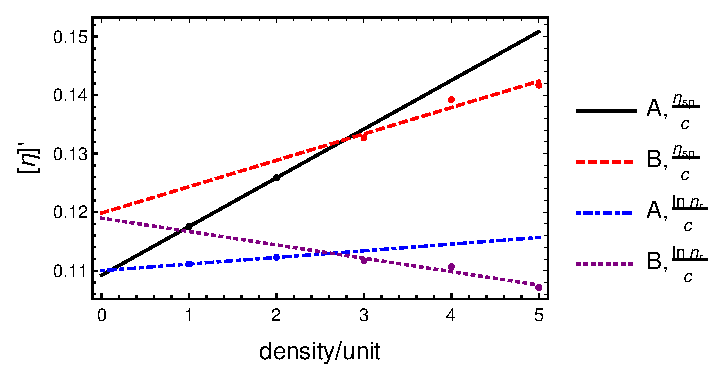
\includegraphics[width=0.4\textwidth]{figures/eta.eps}
\caption{$[\eta]'$-$c$ curves for two groups, two methods}
\label{etafig}
\end{figure}
Group A and group B differs from each other due to different pipes used in the experiment\footnote{It is due to unintentional crack observed in the pipe first used, while limitation of time hinders completion of data.}. 
Different results of $[\eta]$ indicates a strong connection between $\eta$ and the pipes, which seems reasonable with regard to the fact that polyethelene glycol can form strong hydrogen bonds with \ce{SiO2}, which is the main substance of the glass pipe. Different pipes are certain to have different surfaces, and $\eta$ of the solution may thus differ significantly. Two methods calculating $[eta]$ return nearly the same results in each group, validating the data of the experiment. 

Data from Group A gives $14.5\times10^4$ as the polyethelene glycol's viscosity average molecular weight, while it is $16.2\times10^4$ from Group B. 

\section{Acknowledgements}
Special thanks must be given to Zong Wei Huang, who dedicated himself in achieving computational approximation of viscosity of polymer solutions yet did not hesitate to provide enormous help for the realizeation of program and analyses of the results. His work adopting Monte Carlo is certainly impressive, citation of which fais to be included in this report due to limitation of time.
\end{document}
